\subsection{Matcher} \label{sec:matcher}

\subsubsection[Geomatcher]{Geomatcher \myAuthor{Cedric Holzer}}
\label{sec:geo_matcher}

Wir wollen anhand der Formen der Kanten beurteilen, wie gut zwei konkret
rotierte Puzzleteile zusammenpassen. Dazu werden die beiden zu
vergleichenden Kanten zunächst transformiert, um sie hinsichtlich
Position und Orientierung vergleichbar zu machen. Die Größe darf nicht
verändert werden, da die Bilder maßstabsgetreu sind. Jede Kante ist
durch eine zusammenhängende Punktwolke variabler Größe gegeben. Jede
Kante verfügt über zwei Eckpunkte, die beim Einlesen der Kanten
generiert werden. Diese werden aus Sicht des Puzzleteil-Zentrums, also
nach außen blickend, als linke und rechte Ecke bezeichnet.

\paragraph{Vorverarbeitung}

Aus Effizienzgründen werden alle Kanten vorverarbeitet. Pro Kante werden
zwei Punktserien berechnet, die für alle Kanten im gleichen
Koordinatensystem liegen. Es sind zwei Punktserien notwendig, da die zu
vergleichenden Puzzleteile nebeneinander platziert werden müssen. Die
transformierten Punktserien ``liegen'' auf der x-Achse, d.h. ein
Puzzleteil liegt darunter und eines darüber. Jedes Puzzleteil wird für
beide Lagen vorbereitet.

Zunächst werden die Punkte der Kante rotiert, sodass ein Eckpunkt im
Ursprung liegt. Für die unter der x-Achse liegende Position wird hier
der linke Eckpunkt gewählt, für die darüber liegende Position der
rechte. Anschließend werden die Punktwolken um den Ursprung rotiert,
sodass der verbleibende Eckpunkt auf der positiven x-Achse zum Liegen
kommt.

\begin{figure}
\centering
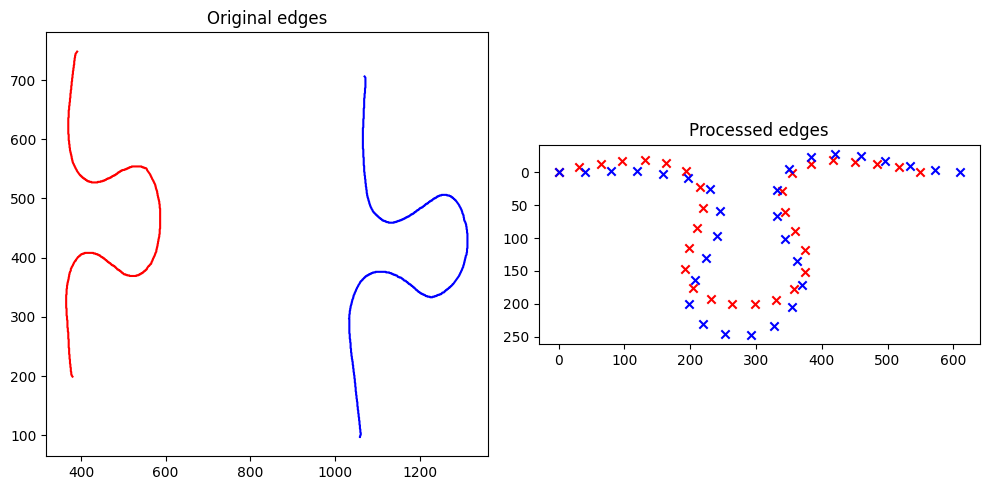
\includegraphics[width=\textwidth]{sections/solver/images/geomatcher_preprocessed_edges.png}
\caption{GeoMatcher Kanten-Vorverarbeitung: Ursprüngliche Kanten im lokalen Bildkoordinatensystem (links) und transformierte Punktwolken (rechts, N=30), die paarweise verglichen werden können.}
\label{fig:geomatcher_preprocessing}
\end{figure}

Anschließend werden die Punktwolken, die unterschiedlich viele Punkte
beinhalten können, durch eine konstante Anzahl von Punkten approximiert.
Dazu wird zunächst die kumulative Kurvenlänge der Kante als dritte
Dimension neben $(x, y)$ eingeführt. Nun werden zwei
Interpolationsfunktionen berechnet, die von der kumulativen Kantenlänge
auf $x$ und $y$ abbilden. Abbildungen $x\rightarrow{}y$ oder $y\rightarrow{}x$ 
sind nicht eindeutig, da die Kante eine nicht-funktionelle Kurve ist. 
Auf der kumulativen Kurvenlänge können $n$ gleichmäßig
verteilte Punkte berechnet und über die vorbereiteten
Interpolationsfunktionen auf $(x, y)$ Koordinaten auf der Kurve abgebildet
werden. Diese Punkte haben jetzt voneinander einen konstanten Abstand,
sind also gleichmäßig über die Kurve verteilt. \autoref{fig:geomatcher_preprocessing} zeigt zwei unterschiedliche Kanten, die jeweils in eigenen lokalen Koordinatensystemen ihres Puzzleteils liegen. Die vorverarbeiteten Versionen liegen einheitlich orientiert auf der positiven x-Achse und wurden durch 30 gleichverteilte Punkte approximiert.

\paragraph{Vergleich}

Um zwei Kanten zu vergleichen, werden für beide Kanten die
vorverarbeiteten Punktwolken abgefragt. \autoref{fig:geomatcher_preprocessing_versions} 
veranschaulicht die beiden unterschiedlichen Versionen einer Kante, die durch die 
Vorverarbeitung entstanden sind. Beim Vergleich ist zu beachten, dass für
eine der Kanten die unter und für die andere Kante die über der x-Achse
liegende Version gewählt werden muss, damit die beiden Teile
zusammenpassen können.  Nun können die beiden Punktwolken gegenläufig
iteriert und die einzelnen Punkte paarweise verglichen werden. Dadurch
lässt sich der Vergleich zweier Kanten auf n Vergleiche zweier Punkte
abbilden. Dieses Framework wird später auch für den GeoMatcherRGB
genutzt.

\begin{figure}
\centering
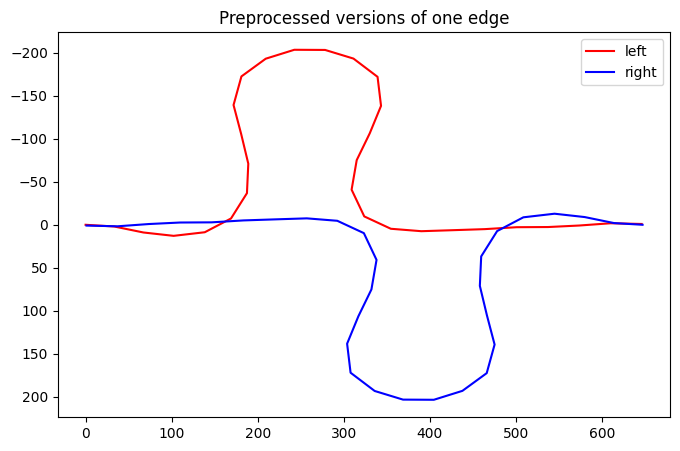
\includegraphics[width=\textwidth]{sections/solver/images/geomatcher_pp_versions.png}
\caption{Beide vorverarbeiteten Punktwolken (interpoliert, N=30) einer einzelnen Kante im GeoMatcher}
\label{fig:geomatcher_preprocessing_versions}
\end{figure}

Sind die beiden Kanten nicht gleich lang, hängt ihre relative
Ausrichtung zueinander und damit der resultierende Match-Score davon ab,
wie die Puzzleteile den beiden Positionen (über und unter der x-Achse)
zugewiesen werden. Das ist unerwünscht, da diese Zuweisung nicht
sinnvoll deterministisch vorgenommen werden kann. Die Lösung besteht
darin, beide möglichen Ausrichtungen zu berechnen und die resultierenden
Scores zu mitteln.

Im Fall des GeoMatchers werden die einzelnen Punkte anhand ihres
euklidischen Abstandes verglichen. Die Abstände aller Punktpaare werden
für die Kante aufsummiert.

\paragraph{Globale Skalierung der Scores}

Die Fehlerwerte der einzelnen Kanten liegen in ${[}0, \infty{[}$, wobei 0
einen perfekten Match darstellt. Gewünscht ist aber eine Darstellung
durch Scores in ${[}0, 1{]}$, wobei 1 einen perfekten Match darstellt.
Daher berechnet der GeoMatcher zu Beginn alle möglichen Matches zwischen
zwei Kanten und skaliert diese mittels $x'\ =\ 1\ -\ (x\ /\ max\_x)$, 
wobei $max\_x$ der höchste im Datensatz vorkommende Match-Score und $x$ der unskalierte
Match-Score ist.

\paragraph{Implementierung}

Der GeoMatcher ist im Package \texttt{algorithm.src.matcher.geo} im solver-Repository 
implementiert. Er nutzt intern ein eigenes Datenmodell, um eine Entkopplung von dem 
volatilen solver-weiten Datenmodell zu erreichen und dieses frei von Matcher-spezifischen
Funktionen zu halten.

\subsubsection[Geomatcher RGB]{Geomatcher RGB  \myAuthor{Simon Hampp}}

\paragraph{Motivation}
In den Farben der Puzzlekanten steckt viel Information, was uns beim Lösen des Puzzles helfen kann. Da unser zu lösendes Puzzle viele Kanten hat, die von der Form her ähnlich aussehen, ist der Farbvergleich wichtig, um diese voneinander zu differenzieren. Die Schwierigkeiten bestand darin, eine effiziente Methode zu finden, die trotzdem alle Farbwerte (RGB) miteinander vergleicht.

\paragraph{Vorgehen}

Die Basis für die Methode zum Vergleichen der Farbe ist der schon implementierte $GeoMatcher$ \autoref{sec:geo_matcher}. Wir hatten die Idee, diesen Matcher zu erweitern, um statt $(x,y)$ Koordinaten der Pfade, die Farbwerte $(r,g,b)$ der Kante zu vergleichen. Der Vorteil hierbei ist, dass die Struktur und viele benötigten Funktionen schon implementiert waren. Lediglich die Methode, um eine Kante zu laden, um sie mit einer anderen zu vergleichen, musste neu implementiert werden. Hier wird dann statt einer Liste von Koordinaten, eine Liste von Farbwerten zurückgegeben.

Die Listen  $\mathbf{p}$  mit den Farbvektoren $\mathbf{p_i}$ zweier Kanten $m$ und $n$ werden dann wie folgt verglichen.

Seien 
\[
\mathbf{p}_i^{\text{m}} = 
\begin{pmatrix}
r_i^{\text{m}} \\
g_i^{\text{m}} \\
b_i^{\text{m}}
\end{pmatrix}
\quad \text{und} \quad
\mathbf{p}_i^{\text{n}} = 
\begin{pmatrix}
r_i^{\text{n}} \\
g_i^{\text{n}} \\
b_i^{\text{n}}
\end{pmatrix}
\]

\[
\text{error} = \frac{1}{n} \sum_{i=1}^{n}  d(\mathbf{p}_i^{m} , \mathbf{p}_i^{n})
\]

wobei

\[
n = \min(\text{len}(\mathbf{p}^{\text{m}}), \text{len}(\mathbf{p}^{\text{n}}))
\]
\[
d() \ \widehat{=} \ \text{euklidische Distanz}
\]


\paragraph{Lösung}

\begin{figure}[h]
    \centering
    \begin{minipage}[b]{0.4\textwidth}
        \centering
        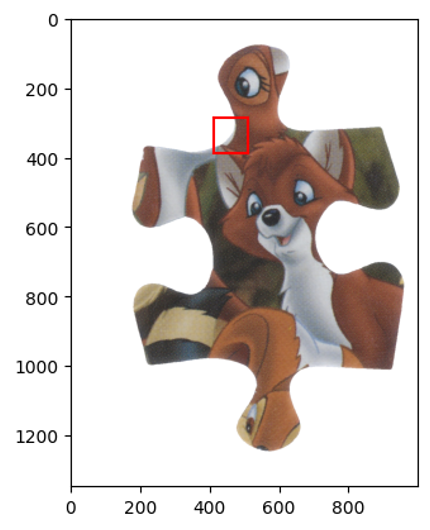
\includegraphics[width=\textwidth]{sections/solver/images/color_piece.png}
        \caption{Beispiel Puzzleteil}
        \label{fig:color_piece}
    \end{minipage}
    \hfill
    \begin{minipage}[b]{0.4\textwidth}
        \centering
        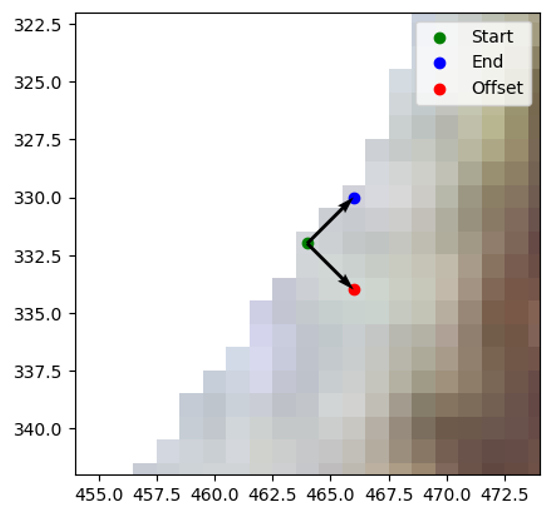
\includegraphics[width=\textwidth]{sections/solver/images/offset.png}
        \caption{Farbextrahierung mit Normalenvektor}
        \label{fig:offset}
    \end{minipage}
    \hfill
\end{figure}

Um die Farbwerte entlang der Kante zu ermitteln, wird diese schrittweise selektiert. Für jeden Pixel $a$ der Kante, für den ein Farbwert generiert werden soll, wird ein Vektor $\mathbf{ab}$ von $a$ zu einem weiteren Punkt $b$ auf der Kante berechnet. Anschließend wird der Normalenvektor $\mathbf{n}_{ab}$ berechnet, der orthogonal auf der Kante bei $a$ steht. Der Farbwert wird dann an der Koordinate $a + \mathbf{n}_{ab}$ ermittelt. Dieses Vorgehen kann man beispielhaft in \autoref{fig:offset} sehen.

Die Methode Normalenvektoren zu generieren für die Kante wurde schon für den ColorMatcher \autoref{sec:color_matcher} benutzt, weshalb auch hier Code wiederverwendet werden konnte.

Bei dem GeoMatcherRGB lassen sich einige Hyperparameter einstellen. Wie viele Farbwerte aus der Kante genommen werden, und wie lang der Normalenvektor ist, und somit wie groß der Abstand zur Kante ist. Diese wirken sich auf die Effektivität des Matchers aus. Um gute Werte zu finden, wurde die Matcher Evaluation \autoref{sec:matcher_evaluation} verwendet. Dabei hat sich herausgestellt, dass es gut ist, viele Farbwerte zu nehmen und nahe (2 Pixel Abstand) an der Kante zu sein. Zu nah an der Kante ist jedoch auch nicht gut, da teilweise Schatten oder Rand an den Kanten ist, der sonst die Auswertung negativ beeinflusst. In der fertigen Lösung, wird für jeden Punkt auf der Kante der Farbwert berechnet, womit alle Kanten des 49-Teile-Puzzles innerhalb von $3.4$ Sekunden verglichen werden können, ohne die Bilder der Puzzleteile zu skalieren.



\subsubsection[ColorMatcher]{ColorMatcher \myAuthor{Maximilian Weigle}}
\label{sec:color_matcher}
Das Farbmatching ist ein Algorithmus, welcher dafür genutzt wird die Ähnlichkeit der Kanten zweier Puzzleteile zu bestimmen. Anders als bei den geometrischen Verfahren werden hierbei die Farbwerte der Pixel an den Kanten für den Vergleich verwendet.

Die Grundannahme für das Verfahren ist, dass, wenn die Farbwerte entlang zweier Kanten möglichst ähnlich zueinander sind, davon ausgegangen werden kann, dass diese Kanten zusammengehören. 

\paragraph{Beschreibung des Verfahrens}
Zunächst muss mithilfe der bereits extrahierten Kanten-Koordinaten, ein Bereich definiert werden, dessen Pixel für den Vergleich verwendet werden. Da sich die Farbwerte entlang einer Kante stark voneinander unterscheiden können, muss diese in mehrere Segmente oder "Patches" aufgeteilt werden, welche dann einzeln miteinander verglichen werden. Die Größe und Anzahl dieser Patches ist konfigurierbar, standardmäßig aber auf 50 gleich große Patches eingestellt, welche jeweils 5 Pixel ins Bild hineinragen (siehe \autoref{fig:color_patches}). Dies entspricht einer ungefähren Größe der Patches von 5x5 Pixeln, was auch von Zhi et al. empfohlen wird \cite{image_matching_color}.

\begin{figure}[H]
    \centering
    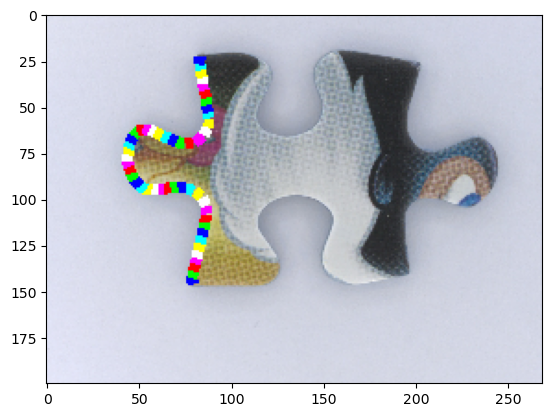
\includegraphics[width=0.75\textwidth]{sections/solver/images/color_patches.png}
    \caption{Farbliche Kennzeichnung der Patches entlang einer Kante}
    \label{fig:color_patches}
\end{figure}

Anschließend wird für jeden dieser Patches ein Histogramm über die Farbwerte bestimmt. Dafür werden, wie in \autoref{fig:color_histograms} zu sehen, die Hue- und Saturation-Komponenten der HSV Darstellung verwendet, da diese die meisten Informationen über einen gleichmäßigen Übergang zwischen der linken und rechten Kante beinhalten. Alternativ kann das Verfahren auch nur in einer Dimension mit den Graustufen-Werten der Bilder verwendet werden, was eine schlechtere Genauigkeit bei besserer Performance mit sich bringt.

Die Verwendung von Histogrammen hat gegenüber anderen Verfahren, wie beispielsweise einem durchschnittlichen Farbwert über alle Pixel, den Vorteil, dass nur tatsächlich existierende Farbwerte in den Vergleich mit aufgenommen werden. Bei zwei sehr kontrastreichen farbigen Flächen innerhalb eines Patch, würde sonst ein Durchschnitt berechnet, welcher im Patch selbst überhaupt nicht vorkommt. 

\begin{figure}[H]
    \centering
    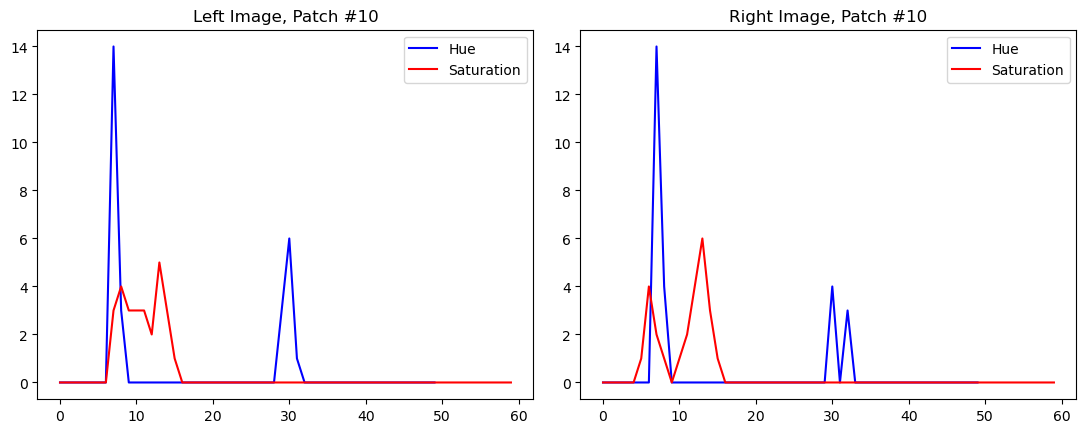
\includegraphics[width=\textwidth]{sections/solver/images/color_histogram.png}
    \caption{Histogramme zweier übereinstimmender Patches}
    \label{fig:color_histograms}
\end{figure}

Im nächsten Schritt werden dann Patch für Patch das Histogramm der rechten mit dem der linken Kante auf Korrelation verglichen. Das Ergebnis hiervon ist ein Wert zwischen 0 und 1, welcher die Ähnlichkeit dieser beiden Patches beschreibt (siehe \autoref{fig:color_matching}).

\begin{figure}[H]
    \centering
    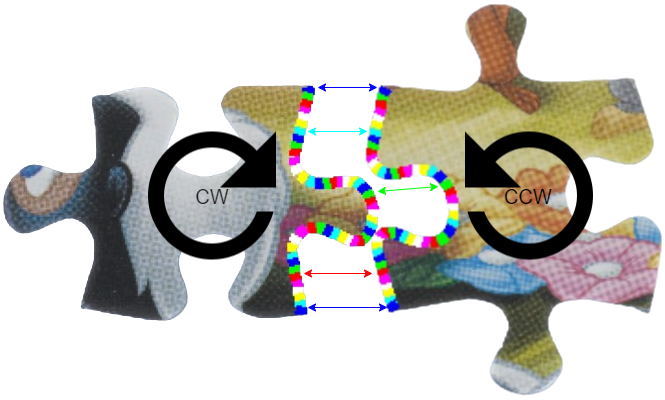
\includegraphics[width=\textwidth]{sections/solver/images/color_matching.png}
    \caption{Vergleich der jeweils korrespondierenden Patches}
    \label{fig:color_matching}
\end{figure}

Wird nun ein Mittelwert über die Korrelationswerte aller Patches bestimmt, dann gibt dieser die Ähnlichkeit der beiden Katen zueinander an. Dieser Wert kann dann an der entsprechenden Stelle in die Match-Matrix eingetragen werden, welche vom Solver Algorithmus verwendet wird um das Puzzle zu lösen.

\paragraph{Größe der Patches}
Die Wahl der Patch-Größe ist sehr wichtig für die Qualität der Ergebnisse. Sie sollen einerseits möglichst klein sein, da dann eine Übereinstimmung der Farbwerte lokal möglichst genau verortet werden kann, die Genauigkeit des Matching also steigt. Andererseits besteht bei zu kleinen Patches die Gefahr, dass Aureißer ein zu hohes Gewicht bekommen. Beispielsweise sind die Fotos oftmals nicht perfekt abgeschnitten, sodass noch ein Streifen grauer Pixel oder ein Schatten am Rand zu sehen ist, der das Ergebnis verfälschen kann. Auch ist es möglich, dass die Ränder der gegenüberliegenden Patches nicht perfekt aufeinander passen, sodass Pixel die eigentlich ins nächste Patch gehören, in den Vergleich mit einfließen. Die Wahl von ungefähr 5 x 5 Pixel großen Patches hat sich bei der gewählten Auflösung der Bilder als guter Kompromiss herausgestellt.

\paragraph{Probleme und Lösungen}
Beim Vergleich der Patches entlang zweier Kanten muss darauf geachtet werden, dass nicht an den entgegengesetzten Enden der aneinander gelegten Kanten begonnen wird. Hierbei ist die Eigenschaft hilfreich, dass die Eck- und Kanten-Koordinaten in ihrer Reihenfolge im PuzzlePiece Objekt stets im Uhrzeigersinn (Clockwise Ordering/CW) abgespeichert werden. Somit müssen an einer der Kanten die Patches in umgekehrter Reihenfolge (damit Counter-Clockwise) iteriert werden, damit die aneinander liegenden Patches miteinander verglichen werden (siehe \autoref{fig:color_matching}).

Durch die Clockwise-Anordnung wird garantiert, dass eine nach rechts zeigende Normale immer ins Puzzleteil "hinein" zeigt. Dies konnte genutzt werden, um bei der Bestimmung der Patches vom Rand ausgehend den Bereich 5 Pixel weit ins Bild zu erweitern.

Die Größe der Bilder von ca. 1000x800 Pixeln war für die Berechnung und den Vergleich vieler Histogramme zu groß und hat die Performance extrem verschlechtert (Berechnung einer Match-Matrix in ca. 30 Minuten). Das Skalieren der Bilder auf 20\% der Größe hat dabei Abhilfe geschaffen, die Berechnungszeit auf nur noch unter 10 Sekunden zu bringen, ohne dabei die Qualität der Matches merklich zu verschlechtern.

Auch die Berechnung der Histogramme musste optimiert werden, um in einer vertretbaren Zeit berechenbar zu sein. Hierfür wurde zunächst die Anzahl der verwendeten Kanäle von 3 (RGB) auf 2 (Hue und Saturation der HSV-Darstellung) reduziert. Außerdem ist es nicht notwendig für alle 256 möglichen Werte eines Farbkanals Bins im Histogramm bereitzustellen. Hier konnten mit 50, bzw. 60 Bins die Übereinstimmung genügend genau festgestellt werden.

\subsubsection[XOR Matcher]{XOR Matcher \myAuthor{Markus Ertl}}
Im folgenden soll die Funktionsweise als auch Einbindung ins Projket des XOR-Matchers genauer betrachtet werden.

\subsubsection*{Grundidee des XOR matchers}

Der XOR-Edge-Matcher basiert auf der Überlagerung der Binärmasken zweier Puzzelkanten \ref{fig:xor_idea}. Ziel ist es, durch Rotation und Verschiebung der Kanten eine minimale Überlappung und den geringsten Leerraum zu erreichen. Diese Methode berücksichtigt ausschließlich geometrische Aspekte des Puzzels, ohne Farben oder Muster der Puzzelteile zu berücksichtigen.

\begin{figure}
    \centering
    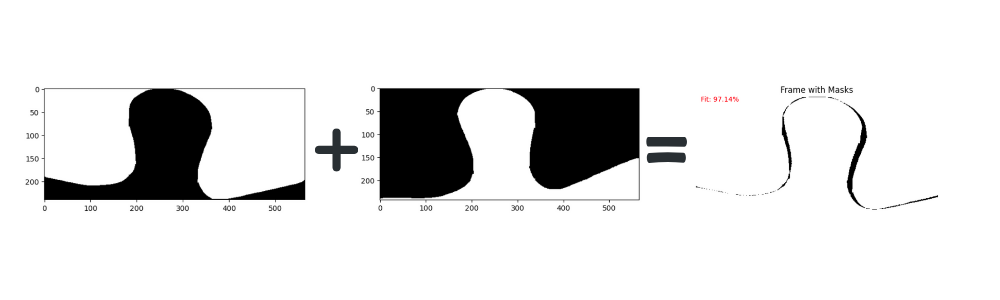
\includegraphics[width=1\linewidth]{sections//solver//images/xor_basic_idea.png}
    \caption{Grundidee des XOR Matchers}
    \label{fig:xor_idea}
\end{figure}

\subsubsection*{Vorbereitung der Daten}

Die Datenvorbereitung umfasst die Umwandlung einer Kantenrepräsentation in eine Binärmaske. Dafür sind mehrere Zwischenschritte notwendig:

\paragraph{1. Normalisierung}
Die Ausrichtung der Kanten variiert. Sie können horizontal oder vertikal mit unterschiedlichen Abständen zum Rand angeordnet sein. Um verwendbare Binärmasken zu generieren, müssen diese Abweichungen normalisiert werden. Dies beinhaltet die Rotation der Kanten um 90°, falls nötig, und die anschließende Verschiebung an den oberen linken Bildrand. Die Notwendigkeit einer Rotation wird durch den Vergleich der Varianz entlang der x- und y-Achse bestimmt:

\[
\operatorname{Var}(x) < \operatorname{Var}(y) \implies \text{vertikale Kante}
\]
\[
\operatorname{Var}(x) > \operatorname{Var}(y) \implies \text{horizontale Kante}
\]
Die Rotation wird durch eine Achsenvertauschung gefolgt von einer Spiegelung entlang der x-Achse durchgeführt:
\[
B = S_x A^T
\]
wobei
\[
S_x = \begin{pmatrix} 1 & 0 \\ 0 & -1 \end{pmatrix}
\]
die Spiegelungsmatrix entlang der x-Achse ist und \( A^T \) die transponierte Matrix von \( A \) darstellt.
Die Matrix \(A\) repräsentiert dabei das Eingangsbild, wobei die Kante mit dem Wert 1 dargestellt wird, und der Rest mit dem Wert 0.

\paragraph{2. Binärmasken}
Die normalisierten Kanten werden anschließend gefüllt. Nach verschiedenen Experimenten mit Techniken wie ``fillPoly'' von OpenCV und ``floodFill'' von scikit-image, wurde ein eigener Füllalgorithmus entwickelt. Die Binärmasken werden von oben nach unten gefüllt, wobei die Kante genau ein Pixel breit sein muss. Ein x-zu-y-Mapping identifiziert den letzten zusammenhängenden weißen Pixel jeder Zeile als Kantenpixel. Der Füllvorgang wechselt die Farbe beim Erreichen einer Kante zwischen Weiß (1) und Schwarz (0). Der Algorithmus wird in Abbildung \ref{alg:maskenfuellung} detaillierter erklärt.
\begin{algorithm}
\caption{Maskenfüllungsalgorithmus}
\label{alg:maskenfuellung}
\begin{algorithmic}[1]
\State \textbf{Input:} BildMaske, KantenMapping
\State \textbf{Output:} GefüllteMaske

\State Initialisiere GefüllteMaske mit den Abmessungen von BildMaske
\State Setze alle Pixel von GefüllteMaske auf 0 (Schwarz)

\For{Jede Spalte $y$ von oben nach unten}
    \State $farbe \gets 1$  \Comment{Startfarbe Weiß}
    \For{Jedes Pixel $x$ in Spalte $y$}
        \If{$x$ ist in KantenMapping für $y$}
            \State $farbe \gets 1 - farbe$  \Comment{Wechselt zwischen 0 und 1}
        \EndIf
        \State Setze Pixel $(x, y)$ in GefüllteMaske auf $farbe$
    \EndFor
\EndFor

\State \textbf{return} GefüllteMaske
\end{algorithmic}
\end{algorithm}

Bei der Auswertung der Ergebnisse wurde festgestellt, dass der Algorithmus Schwierigkeiten bei der Verarbeitung der Scheitelpunkte der Konturen aufweist. Um diese Bildfehler zu korrigieren, wird folgender Ansatz verfolgt: Wenn ein Pixel und seine beiden horizontal benachbarten Pixel unterschiedliche Werte aufweisen, wird das betrachtete Pixel an die Farbe seiner Nachbarn angeglichen.

Der aktuelle Verarbeitungsschritt berücksichtigt nicht, ob es sich bei den Kanten um männliche oder weibliche Typen handelt. Es ist jedoch notwendig, die Binärmaske entsprechend dem im Edge-Objekt definierten Kantentyp anzupassen. Dies geschieht durch die Auswertung der Randpixel: Überwiegen weiße Pixel, handelt es sich vermutlich um eine weibliche Kante; ein Überschuss an schwarzen Pixeln deutet auf eine männliche Kante hin. Stimmt der erkannte Kantentyp nicht mit dem gespeicherten Typ überein, wird das Bild invertiert – weiße Pixel werden schwarz und umgekehrt.

Während des Optimierungsschritts werden die Masken korrekt positioniert und gegebenenfalls leicht rotiert. Hierbei kann ein kleiner schwarzer Rand entstehen, der jedoch nicht als Fehler betrachtet werden sollte. Um mögliche visuelle Störungen zu minimieren, wird zusätzlich ein Padding am Rand der Maske hinzugefügt, um die Darstellung zu verbessern.

\subsubsection*{Optimierung}

Nun geht es um die eigentliche XOR-Optimierung. Dieser Schritt besteht im Grunde aus folgenden sich wiederholenden Schritten:

\paragraph{Masken in Frame platzieren}
Als erstes werden die beiden Binärmasken in einem Frame platziert. Dabei wird die Binärmaske der weiblichen Kante am oberen Rand platziert, und die Maske der männlichen Kante wird so platziert, dass sie bereits etwas mit der weiblichen Binärmaske überlappt. Diese Überlappung wird mit XOR berechnet.

\paragraph{Fit berechnen}
Um nun den Fit zu berechnen werden alle weißen und schwarzen Pixel gezählt. Daraus wird der Score mit dieser Formel berechnet:
\[
1 -  \frac{\left|AnzahlSchwarzerPixel\right|}{\left|AnzahlWeißerPixel\right|}
\]

\paragraph{Verschieben und Rotieren}
Zur Verbesserung des Übereinstimmungsscores wird die Position und Orientierung der Masken durch geringfügiges Verschieben und Rotieren feinjustiert. Dieser Prozess wird so lange fortgesetzt, bis keine weitere Verbesserung des Scores möglich ist, was auf das Erreichen eines lokalen Minimums hinweist. In idealen Fällen entspricht dieses lokale Minimum einem globalen Minimum, allerdings ist die Überprüfung dieser Annahme zeitintensiv und nicht unmittelbar realisierbar.

\subsubsection*{Einbindung in Solver}
Der XOR-Optimierer ist, wie auch die anderen Matcher, über das Matcher-Interface in das Projekt integriert. 

\subsubsection*{Bewertung des Matchers}
Die Auswertung des Beispiel-Puzzles zeigte, dass der XOR-Optimierer nur teilweise korrekte Ergebnisse liefert. Die isolierte Betrachtung einer Kante erweist sich nicht als ausreichend einzigartig, um verlässlich vorherzusagen, ob zwei Puzzleteile zusammengehören. Eine mögliche Verbesserung der Vorhersagegenauigkeit könnte durch die Kombination des XOR-Matchers mit einem Farb-Matcher erreicht werden.

\subsubsection[Evaluierung]{Evaluierung \myAuthor{Cedric Holzer}}
\label{sec:matcher_evaluation}

Um die Leistung unserer Matcher vergleichen sowie optimale Hyperparameter finden 
zu können, ist eine objektive Beurteilung ihrer Güte notwendig. Dazu werden im
Folgenden verschiedene Metriken untersucht.

Dieses Kapitel nutzt eine händische gefundene Lösung des Puzzles als
Referenz. Für jede Kante ist also der korrekte Partner bekannt.

\paragraph{Binärer Prediktor}

Die Matcher können als binäre Klassifikatoren interpretiert werden.
Dafür werden zunächst alle Kanten miteinander verglichen. Für jede Kante
wird dann diejenige Partner-Kante ausgewählt, die den besten
Matcher-Score erreichte. Dadurch wird für jede Kante so ein Partner als
``passend'' prädiziert, während alle anderen Kantenpaare als
``unpassend'' prädiziert werden.

Mit dieser Interpretation lassen sich anschließend gängige Metriken für
binäre Klassifikatoren anwenden. Dazu zählt man zunächst die Anzahl der
richtigerweise als passend ($tp$) und unpassend ($tn$) und
fälschlicherweise als passend ($fp$) bzw. unpassend ($fn$)
prädizierten Kantenpaaren, stellt also eine Konfusionsmatrix auf. Darauf
aufbauend berechnet man die in \autoref{tab:matcher_eval_metrics} beschriebenen Metriken.

\begin{table}
    \centering
    \begin{tabular}{||ccp{0.6\textwidth}||}
        \hline
        Metrik & Berechnung & Interpretation \\
        \hline\hline
        Accuracy     & $\frac{tp + tn}{tp + tn + fp + fn}$ & Anteil aller korrekt prädizierten Kantenpaare                                                  \\
        Precision    & $\frac{tp}{tp + fp}$ & Wahrscheinlichkeit, mit der ein als passend prädiziertes Kantenpaar tatsächlich passend ist.   \\
        Recall       & $\frac{tp}{tp + fn}$ & Wahrscheinlichkeit, mit der ein tatsächlich passendes Kantenpaar als solches prädiziert wird.  \\
        F1-Score     & $\frac{2 * tp}{2 * tp + fp + fn}$ & Kombination aus Precision und Recall                                                          \\
        Specificity  & $\frac{tn}{tn + fp}$ & Wahrscheinlichkeit, mit der ein unpassendes Kantenpaar als solches prädiziert wird.            \\
        \hline
    \end{tabular}
    \caption{Gängige Metriken zur Beurteilung der Leistung von binären Klassifikatoren}
    \label{tab:matcher_eval_metrics}
\end{table}

Die Metriken Precision, Recall und F1-Score sind dabei redundant, da das
vorliegende Problem eine besondere Form hat: Pro Kante wird genau ein
Kantenpaar als passend prädiziert. Wird ein unpassendes Kantenpaar
fälschlicherweise als passend prädiziert, so kann das tatsächlich
passende Kantenpaar nicht auch noch als passend prädiziert werden. Die
Anzahl der falsch klassifizierten Kantenpaare ist also für beide Label
gleich, es gilt $fp=fn$.

\paragraph{Trennschärfe}

Ein zusätzlicher Ansatz zur Beurteilung der Aussagekraft eines
Matchers ist die Trennschärfe, die anders als die Betrachtung der binären Klassifikatoren
auch die exakten Match-Scores berücksichtigt. Dazu wurde für
jede Kante die Differenz aus dem Matcher-Score des passenden
Kantenpaares und dem höchsten Matcher-Score eines unpassenden
Kantenpaares gebildet. Diese Metrik wird im nachfolgenden als absolute
Trennschärfe (selectiveness) bezeichnet. Sie nimmt Werte in ${[}-1,1{]}$ an, wobei ein Wert 
von -1 bedeuten würde, dass passende Kantenpaare immer
einen schlechten Score von 0 erhalten, während mindestens ein
unpassendes Kantenpaar den Wert 1 erhält. Ein Wert von 0 wäre mit einem
konstanten Matcher-Score trivial erreichbar und ein Wert von 1 wäre
perfekt: Passende Kantenpaare hätten einen Score von 1, während alle
unpassenden Kantenpaare einen Score von 0 erhalten.

Die relative Trennschärfe wird gebildet, indem der absolute
Trennschärfe-Wert durch den Score des besten unpassenden Kantenpaares
geteilt wird.

\paragraph{Kombinationen von Matchern}

Mehrere Matcher können kombiniert werden, indem sie unabhängig
voneinander Match-Scores für ein Kantenpaar errechnen und das Produkt
der einzelnen Scores als Gesamtscore gewertet wird. Das Bilden des
Produktes übergewichtet niedrige Scores dahingehend, dass ein einziger
sehr niedriger Einzelscore ausreicht, um den Gesamtscore stark zu
senken, selbst wenn viele andere Einzelscores sehr hoch sind. Dieses
Vorgehen basiert auf der Annahme, dass korrekte Kantenpaare von jedem
Matcher einen recht hohen Score erhalten. Inkorrekte Kantenpaare
erhalten aber tendenziell von mindestens einem Matcher einen
schlechteren Score und werden so stärker aussortiert, selbst wenn die
anderen Einzelmatcher sie nicht von dem korrekten Kantenpaar hätten
unterscheiden können.

Kombiniert man einen einzigen Matcher mit sich selbst, entspricht dies
einer Potenzierung des Scores. Dabei sinken niedrige Scores schneller
als hohe, die Trennschärfe steigt automatisch. So hat beispielsweise der
GeoMatcher eine absolute Trennschärfe von $0.049$. Kombiniert man ihn
jedoch mit sich selbst, erreicht er auf einmal einen Wert von $0.087$ bei
identischen Werten für die Metriken der binären Klassifikation. Der
Matcher scheint sich also zu verbessern, ohne dass zusätzliche
Informationen oder Fähigkeiten eingeflossen sind. Um daher die
nachfolgenden Ergebnisse vergleichbar zu machen, wird stets eine
Kombination aus vier Matchern evaluiert. Sind weniger Matcher vorhanden,
werden diese mehrfach verwendet. Die Potenzen über den Matchernamen
zeigen die Gewichtung der Matcher an.

\paragraph{Ergebnisse}

\subparagraph{Formbasierte Matcher}

\begin{table}
    \centering
    \begin{tabular}{||c|ccc||}
        \hline
        Metrik & Geo\textsuperscript{4} & XOR\textsuperscript{4} & Geo\textsuperscript{2}$\cdot$XOR\textsuperscript{2} \\
        \hline\hline
        Accuracy                                 & 99.83\% & 97.71\%   & 99.55\%  \\
        Precision / Recall                       & 92.86\% & 5.95\%    & 81.55\%  \\
        Specificity                              & 99.91\% & 98.84\%   & 99.77\%  \\
        $\not\!\circ \;$ Trennschärfe (absolut)  & 0.139   & -0.109    & 0.057   \\
        $\not\!\circ \;$ Trennschärfe (relativ)  & 27.81\%  & -17.67\%  & 12.24\%  \\
        $\not\!\circ \;$ Matcher-Score           & 0.085   & 0.139     & 0.102   \\
        \hline
    \end{tabular}
    \caption{Matcher Evaluation für formbasierte Matcher}
    \label{tab:matcher_eval_shape}
\end{table}

\autoref{tab:matcher_eval_shape} zeigt die Evaluationsresultate für die formbasierten Matcher, nämlich den Geo- und XOR-Matcher. Beide sind nicht in der Lage, alle Puzzleteile
korrekt zu prädizieren. Der GeoMatcher klassifiziert zumindest den
überwiegenden Teil der Kantenpaare korrekt und erreicht so eine
Precision von 92.86\% bei relativ niedriger, aber positiver
Trennschärfe. Der XOR-Matcher scheitert beim Großteil der Kanten daran,
dem passenden Kantenpaar den jeweils höchsten Score zu verleihen.
Dementsprechend ist auch die Trennschärfe hier negativ. Eine Kombination
der beiden Matcher liefert keinen Mehrwert und erreicht das Ergebnis des
GeoMatchers nicht.

\subparagraph{Farbbasierte Matcher}

\begin{table}
    \centering
    \begin{tabular}{||c|ccc||}
        \hline
        Metrik & RGB\textsuperscript{4} & Color\textsuperscript{4} & RGB\textsuperscript{2}$\cdot$Color\textsuperscript{2} \\
        \hline\hline
        Accuracy                                 & 100.00\% & 99.94\%  & 100.00\%  \\
        Precision / Recall                       & 100.00\% & 97.62\%  & 100.00\%  \\
        Specificity                              & 100.00\% & 99.97\%  & 100.00\%  \\
        $\not\!\circ \;$ Trennschärfe (absolut)  & 0.177   & 0.017   & 0.063    \\
        $\not\!\circ \;$ Trennschärfe (relativ)  & 71.25\%  & 360.46\% & 209.28\%  \\
        $\not\!\circ \;$ Matcher-Score           & 0.042   & 0.000   & 0.004    \\
        \hline
    \end{tabular}
    \caption{Matcher Evaluation für farbbasierte Matcher}
    \label{tab:matcher_eval_color}
\end{table}

Wie in \autoref{tab:matcher_eval_color} erkennbar schneiden die beiden farbbasierten 
Matcher GeoMatcherRGB und ColorMatcher deutlich besser als die formbasierten ab. 
Der GeoMatcherRGB kann alleine bereits alle
Kantenpaare korrekt prädizieren und erreicht perfekte Accuracy-,
Precision- und Specificity-Werte. Zeitgleich zeigt er eine bessere
Trennschärfe als der GeoMatcher.

Der ColorMatcher prädiziert einige wenige Kantenpaare inkorrekt, schlägt
die formbasierten Matcher aber dennoch. Er verfügt über eine sehr
niedrige absolute Trennschärfe. Generell erzeugt er sehr niedrige
Scores, die durch die Potenzierung stark verringert werden. Dies schlägt
sich auch im Durchschnitt der Scores nieder und erzeugt so eine sehr
hohe relative Trennschärfe.

In Kombination können beide Matcher alle Kantenpaare richtig
prädizieren. Die hohe Genauigkeit des GeoMatcherRGBs wird beibehalten,
aber der ColorMatcher sorgt auch hier für deutlich niedrigere Scores und
damit eine hohe relative Trennschärfe. Ein realer Mehrwert dieser
Kombination über den GeoMatcherRGB ist schwer zu beurteilen.

\subparagraph{Kombination von farb- und formbasierten Matchern}

\begin{table}
    \centering
    \begin{tabular}{||c|ccc||}
        \hline
        Metrik & Geo\textsuperscript{2}$\cdot$RGB\textsuperscript{2} & Geo\textsuperscript{2}$\cdot$Color\textsuperscript{2} & Geo\textsuperscript{2}$\cdot$RGB$\cdot$Color \\
        \hline\hline
        Accuracy                                 & 100.00\% & 100.00\% & 100.00\%     \\
        Precision / Recall                       & 100.00\% & 100.00\% & 100.00\%     \\
        Specificity                              & 100.00\% & 100.00\% & 100.00\%     \\
        $\not\!\circ \;$ Trennschärfe (absolut)  & 0.259   & 0.086     & 0.165      \\
        $\not\!\circ \;$ Trennschärfe (relativ)  & 85.10\%  & 241.86\% & 173.83\%    \\
        $\not\!\circ \;$ Matcher-Score           & 0.053   & 0.005     & 0.016     \\
        \hline
    \end{tabular}
    \caption{Matcher Evaluation für farb-/formbasierte Matcher kombiniert}
    \label{tab:matcher_eval_color_shape}
\end{table}

Eine Kombination von form- und farbbasierten Matchern ist
vielversprechend, weil so Kanten ähnliche Formen und Farben haben
müssten, um fälschlicherweise hohe Scores zu erhalten. So sollte sich in vielen Fällen, in denen ein einzelner Matcher mehrere Kandidaten liefert, das passende Kantenpaar erkennen lassen. Die Ergebnisse der Evaluation sind in \autoref{tab:matcher_eval_color_shape} dargestellt.

\begin{figure}
\centering
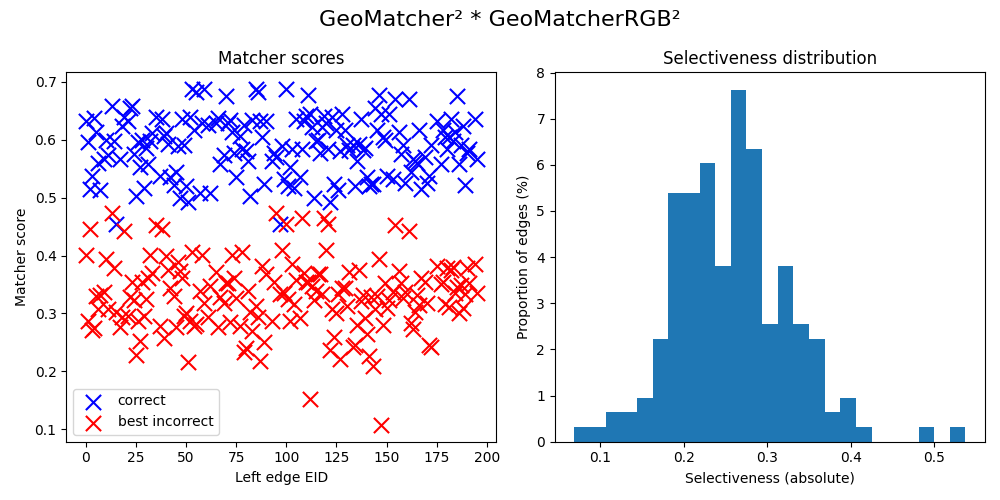
\includegraphics[width=\textwidth]{sections/solver/images/scores_geo2_rgb2.png}
\caption{Matcher-Scores und Verteilung der Trennschärfe für Kombination aus GeoMatcher und GeoMatcherRGB}
\label{fig:matcher_scores_geo}
\end{figure}

In Kombination mit dem GeoMatcher können beide farbbasierten Matcher
alle Kantenpaare richtig prädizieren.  Die Trennschärfe der Kombination mit dem ColorMatcher übersteigt trotz eines höheren durchschnittlichen Scores die Werte, die die Kombination der beiden farbbasierten Matcher erreichen konnte. \autoref{fig:matcher_scores_geo} zeigt die Verteilung der Matcher-Scores für die Kombination aus GeoMatcher und GeoMatcherRGB für jeweils passende und unpassende Kantenpaare. Dabei zeigt sich eine deutliche Separierung in fast linear trennbare Punktwolken. 

In Kombination mit dem XOR-Matcher (nicht dargestellt) ist weder der ColorMatcher noch der GeoMatcherRGB in der Lage, alle Kantenpaare korrekt zu klassifizieren.

\subparagraph{Schlussfolgerungen}

Der GeoMatcherRGB ist der leistungsstärkste Einzelmatcher, der im Rahmen
des Projekts entwickelt wurde. Der GeoMatcher ist eine sinnvolle
Kombination, um neben der Farbe auch die Form von Kanten als zweite
Komponente zu berücksichtigen. Der ColorMatcher wirkt sich vor allem
stark senkend auf die Durchschnittswerte der Scores aus und lässt so die
relative Trennschärfe ansteigen. Ob er darüber hinaus Vorteile bietet,
lässt sich mit dem vorhandenen Datensatz nicht sagen. \autoref{fig:matcher_scores_all} zeigt die Matcher-Scores und die Verteilung der absoluten Trennschärfe für eine Kombination aus GeoMatcher, GeoMatcherRGB und ColorMatcher. Es zeigt sich eine ähnlich starke Ausbildung nahezu linear separierbarer Punktwolken wie in \autoref{fig:matcher_scores_geo}, wobei die Scores durch den ColorMatcher insgesamt in einen niedrigeren Wertebereich gedrückt werden. Der XorMatcher ist den anderen Matchern deutlich unterlegen. Insgesamt empfiehlt sich damit die Anwendung eine Kombination aus GeoMatcher und GeoMatcherRGB, die gegebenenfalls
mit dem ColorMatcher ergänzt werden kann.

\begin{figure}
\centering
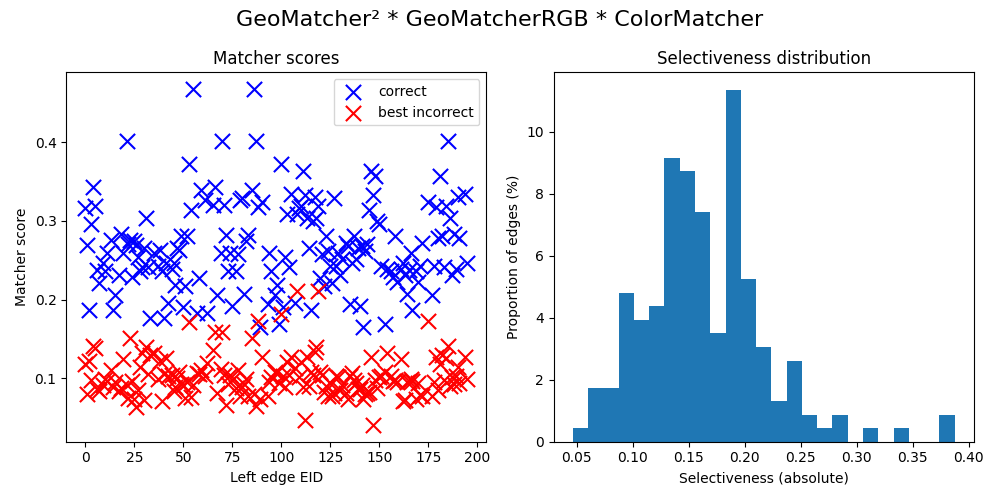
\includegraphics[width=\textwidth]{sections/solver/images/scores_geo2_rgb_color.png}
\caption{Matcher-Scores und Verteilung der Trennschärfe für Kombination aus GeoMatcher, GeoMatcherRGB und ColorMatcher}
\label{fig:matcher_scores_all}
\end{figure}

\paragraph{Implementierung}

Die Evaluation der Matcher ist im solver-Repository im package
\texttt{src.evaluation.matchers} implementiert. Dort findet sich auch
ein entsprechendes Jupyter-Notebook, in welchem die Evaluation im Detail nachvollzogen werden kann.

